\newpage
\section{Other Findings}
\label{sec:other-findings}

Even though the results from the previous Section~\ref{sec:fides-resilience} suggest that a combination of $DistanceBasedTIEvaluation$ for evaluating the interactions in combination with $AverageConfidenceTIAggregation$ is the best, this is not always true.

For example, recall Figure~\ref{fig:single-simulation-example} from Section~\ref{sec:general-overview-of-simulation-output}, where the presented situation uses $MaxConfidenceTIEvaluation$ and it is able to correctly detect all types of peers as well as correctly determine the score for the target.
However, if we take the same environment and the only difference is using $DistanceBasedTIEvaluation$ for evaluating interactions, we get the following graph for the service trust in  Figure~\ref{fig:zero-gained-trust}. The graph for confidence as well as target score for the situation from Figure~\ref{fig:zero-gained-trust} can be seen in the appendix in the Figure~\ref{fig:zero-gained-trust-all}.

\begin{figure}[ht]
    \centering
    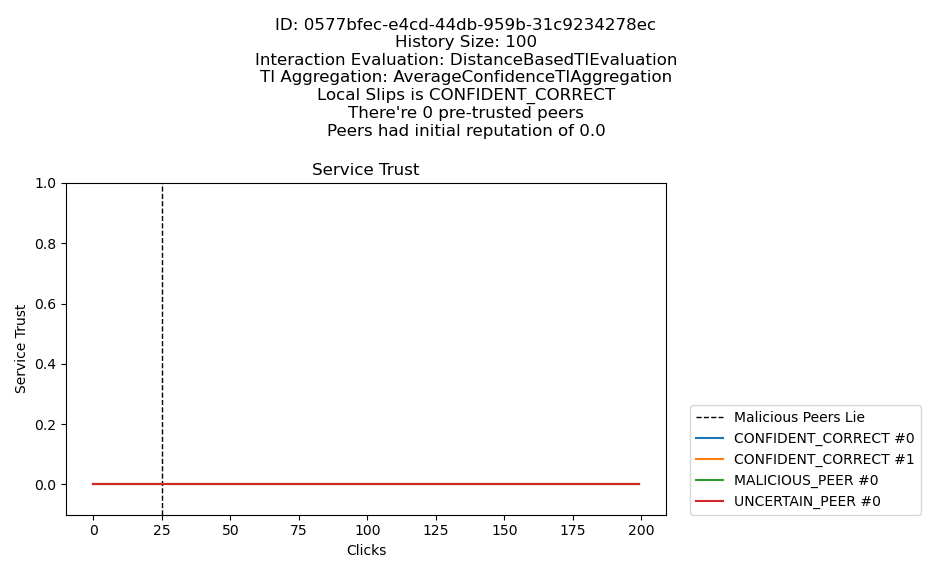
\includegraphics[width=0.8\textwidth]{assets/zero_gained_trust.png}
    \caption{$DistanceBasedTIEvaluation$ in the situation from the figure~\ref{fig:single-simulation-example}}
    \label{fig:zero-gained-trust}
\end{figure}

The service trust graph in Figure~\ref{fig:zero-gained-trust} suggests that Fides didn't gain any trust for any peer in the network.
This happens because the evaluation strategy didn't have enough information at the beginning to evaluate the received data properly.
That leads to peers never gaining any trust and thus not producing any valid outputs because, with no trust, the target score and confidence ended up being $0$ as well.